\documentclass{article}
\usepackage[utf8]{inputenc}
\usepackage{graphicx}
\usepackage{float}
\usepackage{amsmath}
\usepackage[paper=a4paper,margin=1in]{geometry}
\usepackage[table,xcdraw]{xcolor}
\usepackage{url}

\title{Audio analysis and feature extraction}
\author{David Štych\\ Aleksandra Jamróz}
\date{\today{}}



\begin{document}
\maketitle

\section*{Introduction}
%TODO some bullshit useless intro here


\section*{Feature extraction}
On top of the baseline implementation we added another three features. The five features we used are:
\begin{enumerate}
%1
\item \textit{Average value of the entropy of the energy of the audio signal’s frames}
\begin{itemize}
\item Included in the baseline code
\end{itemize}
%2
\item \textit{Maximum value of the entropy of the energy of the audio signal’s frames}
\begin{itemize}
\item Included in the baseline code
\end{itemize}
%3
\item \textit{Average value of the spectral entropy of the audio signal’s frames}
\begin{itemize}
\item Implemented in the provided code
%TODO some justification here por favor
\end{itemize}
%4
\item \textit{Average value of the spectral flux of the audio signal’s frames}
\begin{itemize}
\item Implemented in the provided code
%TODO some justification here por favor
\end{itemize}
%5
\item \textit{Average value of the zero crossing rates of the audio signal’s frames}
\begin{itemize}
\item Implemented in the provided code
%TODO some justification here por favor
\end{itemize}


\end{enumerate}

We have also tried experimenting with other features. We have tried adding \textit{maximum value of the zero crossing rate of the audio signal’s frames} and \textit{average value of the spectral contrast of the audio signal’s frames}. However, in both cases a detremental effect was observed, so we decided not to include them in our model.


\section*{Results}
We kept the default split ration in the dataset (70\% training, 30\% testing). Firstly, we kept the default parameters (frame length, number of subframes and hop length) and just experimented with the features. We tracked the progress and recorded the results in the table below.


\begin{table}[H]
\centering
\begin{tabular}{|
>{\columncolor[HTML]{FFFFFF}}l |
>{\columncolor[HTML]{FFFFFF}}c |}
\hline
\multicolumn{1}{|c|}{\cellcolor[HTML]{C0C0C0}{\color[HTML]{000000} \textbf{Features}}}                                                                                                                        & \cellcolor[HTML]{C0C0C0}{\color[HTML]{000000} \textbf{AUC}} \\ \hline
\cellcolor[HTML]{FFFFFF}{\color[HTML]{000000} Baseline}                                                                                                                                                       & {\color[HTML]{000000} 0.486}                                \\ \hline
{\color[HTML]{000000} \begin{tabular}[c]{@{}l@{}}Baseline\\ Mean of spectral entropies\end{tabular}}                                                                                                          & {\color[HTML]{000000} 0.554}                                \\ \hline
{\color[HTML]{000000} \begin{tabular}[c]{@{}l@{}}Baseline\\ Mean of spectral entropies\\ Mean of spectral flux\end{tabular}}                                                                                  & {\color[HTML]{000000} 0.577}                                \\ \hline
{\color[HTML]{000000} \textbf{\begin{tabular}[c]{@{}l@{}}Baseline\\ Mean of spectral entropies\\ Mean of spectral flux\\ Mean of zero crossing rate\end{tabular}}}                                            & {\color[HTML]{000000} \textbf{0.6}}                         \\ \hline
\cellcolor[HTML]{FFFFFF}{\color[HTML]{000000} \begin{tabular}[c]{@{}l@{}}Baseline\\ Mean of spectral entropies\\ Mean of spectral flux\\ Mean of zero crossing rate\\ Max of zero crossing rate\end{tabular}} & {\color[HTML]{000000} 0.588}                                \\ \hline
{\color[HTML]{000000} \begin{tabular}[c]{@{}l@{}}Baseline\\ Mean of spectral entropies\\ Mean of spectral flux\\ Mean of zero crossing rate\\ Mean of spectral contrast\end{tabular}}                         & {\color[HTML]{000000} 0.583}                                \\ \hline
\end{tabular}
\end{table}


After we have decided which features to use, an automatic algorith was implemented to tune the parameters of the feature engineering. Sets of three parameters are defined in a list and a function goes through the list and tries to train and test the model. AUC is calculated and stored in another list. After completion the set of parameters with the highest AUC is selected. Effect of the parameter change can be seen in the table below.

Best parameters found were:
\begin{itemize}
\item Frame length: 1024
\item Number of subframes: 8
\item Hop length: 256
\end{itemize}
\begin{table}[H]
\centering
\begin{tabular}{|
>{\columncolor[HTML]{FFFFFF}}c |
>{\columncolor[HTML]{FFFFFF}}c |
>{\columncolor[HTML]{FFFFFF}}c |
>{\columncolor[HTML]{FFFFFF}}c |}
\hline
\cellcolor[HTML]{C0C0C0}{\color[HTML]{000000} \textbf{Frame length}} & \cellcolor[HTML]{C0C0C0}{\color[HTML]{000000} \textbf{Number of subframes}} & \cellcolor[HTML]{C0C0C0}{\color[HTML]{000000} \textbf{Hop length}} & \cellcolor[HTML]{C0C0C0}{\color[HTML]{000000} \textbf{AUC}} \\ \hline
\cellcolor[HTML]{FFFFFF}{\color[HTML]{000000} 512}                   & \cellcolor[HTML]{FFFFFF}{\color[HTML]{000000} 10}                           & \cellcolor[HTML]{FFFFFF}{\color[HTML]{000000} 128}                 & {\color[HTML]{000000} 0.6004}                               \\ \hline
{\color[HTML]{000000} 512}                                           & {\color[HTML]{000000} 10}                                                   & \cellcolor[HTML]{FFFFFF}{\color[HTML]{000000} 256}                 & {\color[HTML]{000000} 0.5944}                               \\ \hline
{\color[HTML]{000000} 512}                                           & \cellcolor[HTML]{FFFFFF}{\color[HTML]{000000} 8}                            & {\color[HTML]{000000} 128}                                         & {\color[HTML]{000000} 0.6050}                               \\ \hline
{\color[HTML]{000000} 512}                                           & \cellcolor[HTML]{FFFFFF}{\color[HTML]{000000} 8}                            & {\color[HTML]{000000} 256}                                         & {\color[HTML]{000000} 0.5541}                               \\ \hline
\cellcolor[HTML]{FFFFFF}{\color[HTML]{000000} 1024}                  & {\color[HTML]{000000} 10}                                                   & {\color[HTML]{000000} 128}                                         & {\color[HTML]{000000} 0.5399}                               \\ \hline
{\color[HTML]{000000} 1024}                                          & {\color[HTML]{000000} 10}                                                   & {\color[HTML]{000000} 256}                                         & {\color[HTML]{000000} 0.5794}                               \\ \hline
{\color[HTML]{000000} 1024}                                          & {\color[HTML]{000000} 8}                                                    & {\color[HTML]{000000} 128}                                         & {\color[HTML]{000000} 0.6409}                               \\ \hline
{\color[HTML]{000000} \textbf{1024}}                                 & {\color[HTML]{000000} \textbf{8}}                                           & {\color[HTML]{000000} \textbf{256}}                                & {\color[HTML]{000000} \textbf{0.6424}}                      \\ \hline
\end{tabular}
\end{table}

\begin{figure}[H]
\centering
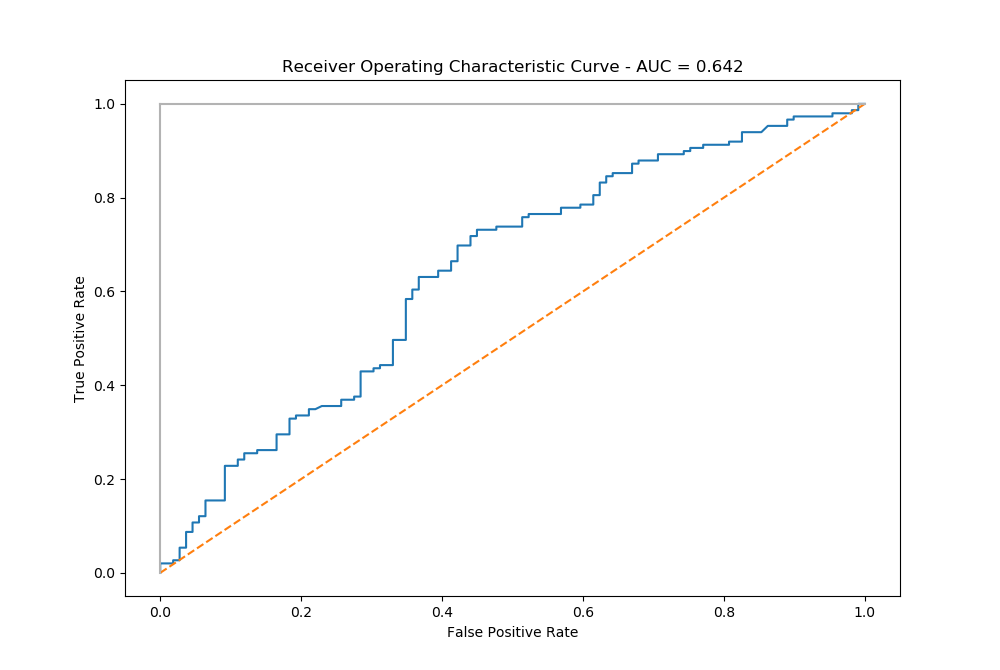
\includegraphics[width=0.8\textwidth]{figures/best_result.png}
\caption{Best result achieved}
\end{figure}



\end{document}

